\documentclass[11pt]{article}
\usepackage{ucs}
\usepackage[utf8x]{inputenc}
\usepackage{changepage}
\usepackage{graphicx}
\usepackage{amsmath}
\usepackage{gensymb}
\usepackage{amssymb}
\usepackage{enumerate}
\usepackage{tabularx}
\usepackage{lipsum}

\oddsidemargin 0.0in
\evensidemargin 0.0in
\textwidth 6.27in
\headheight 1.0in
\topmargin 0.0in
\headheight 0.0in
\headsep 0.0in
%\textheight 9.69in
\textheight 9.00in

\setlength\parindent{0pt}

\newenvironment{myenv}{\begin{adjustwidth}{0.4in}{0.4in}}{\end{adjustwidth}}
\renewcommand{\abstractname}{Anotācija}
\renewcommand\refname{Atsauces}

\newenvironment{uzdevums}[1][\unskip]{%
\vspace{3mm}
\noindent
\textbf{#1:}
\noindent}
{}

\newcommand{\subf}[2]{%
  {\small\begin{tabular}[t]{@{}c@{}}
  #1\\#2
  \end{tabular}}%
}



\newcounter{alphnum}
\newenvironment{alphlist}{\begin{list}{(\Alph{alphnum})}{\usecounter{alphnum}\setlength{\leftmargin}{2.5em}} \rm}{\end{list}}


\makeatletter
\let\saved@bibitem\@bibitem
\makeatother

\usepackage{bibentry}
%\usepackage{hyperref}

%\title{}
%\author{\vspace{-10ex}\mbox{aa}}
%\date{2016-09-19}

\author{\mbox{}\hspace{1ex}\vspace{-4ex}% Toggle commenting out the command
}
\date{2016-09-19}
\title{Testi skaitļu teorijā, 7.--8.klase\vspace{-4ex}% to see the effect
}



\begin{document}

\maketitle

\section{Dalāmības ievads. \texttt{nt.div}}

%% PAŅEMTS uz DUDAJEVAGATVE.LV
\begin{uzdevums}[nt.divisibility.01]
% AOPS.INT.1.1
Cik daudzi pozitīvi trīsciparu skaitļi dalās gan ar 11, gan ar 5? 
\end{uzdevums}


\begin{uzdevums}[nt.divisibility.02]
% AOPS.INT.1.2
Kurš ir mazākais pozitīvais skaitļa 25 daudzkārtnis, kura ciparu reizinājums arī ir pozitīvs skaitļa 25 daudzkārtnis?
\end{uzdevums}


\begin{uzdevums}[nt.divisibility.03]
% AOPS.INT.1.3
Kuri no apgalvojumiem ir patiesi?
\begin{enumerate}[A.]
\item 3 ir skaitļa 18 dalītājs.
\item 17 ir skaitļa 187 dalītājs, bet nav skaitļa 52 dalītājs.
\item 24 nav ne skaitļa 72, ne arī skaitļa 67 dalītājs.
\item 13 ir 26 dalītājs, bet nav 52 dalītājs. 
\item 8 ir skaitļa 160 dalītājs.
\end{enumerate}
{\em  Pierakstiet savu atbildi ar burtiem alfabētiskā secībā, atdalot burtus ar komantiem. Piemēram, ja uzskatāt, ka visi pieci apgalvojumi ir patiesi, rakstiet "A,B,C,D,E" (bez pēdiņām).}
\end{uzdevums}


\begin{uzdevums}[nt.divisibility.04]
% AOPS.INT.1.4
Visi skaitļa 175 pozitīvie dalītāji, izņemot 1, ir izrakstīti pa apli tā, ka jebkuriem diviem skaitļiem 
blakus uz apļa ir kopīgs reizinātājs, 
kas lielāks par 1. Kāda ir summa abiem skaitļiem, kuri uzrakstīti blakus skaitlim 7?
\end{uzdevums}



\begin{uzdevums}[nt.divisibility.05]
% AOPS.INT.1.5
Orķestrī spēlē 72 skolēni, kuri visi soļos sporta spēles pārtraukumā. Viņiem jāsoļo rindās -- ar vienādu skolēnu skaitu katrā rindā. 
Vienā rindā jābūt 5--20 skolēniem. Cik dažādus rindu garumus orķestra dalībnieki var izveidot?
\end{uzdevums}


\begin{uzdevums}[nt.divisibility.06]
% AOPS.INT.1.6
Pieņemsim, ka $a$ un $b$ ir veseli pozitīvi skaitļi, kur skaitlim $a$ ir 3 dalītāji, bet skaitlim $b$ ir $a$ dažādi dalītāji. 
Ja $b$ dalās ar $a$, tad kāda var būt skaitļa $b$ mazākā iespējamā vērtība? 
\end{uzdevums}


\begin{uzdevums}[nt.divisibility.07]
% AOPS.INT.1.7
Kāds ir lielākais veselais skaitlis, ar kuru dalās jebkuru trīs pēc kārtas sekojošu naturālu skaitļu reizinājums? 
\end{uzdevums}


\begin{uzdevums}[nt.divisibility.08]
% AOPS.INT.1.8
Naturāli skaitļi $A,$ $B,$ $A-B$ un $A+B$ visi ir pirmskaitļi. Šo četru pirmskaitļu summa ir\\
{\bf (A)} pāra skaitlis;\hspace{1ex} {\bf (B)} dalās ar $3$;\hspace{1ex} {\bf (C)} dalās ar $5$;\hspace{1ex} 
{\bf (D)} dalās ar $7$;\hspace{1ex} {\bf (E)} ir pirmskaitlis\\
{\em Pierakstiet savu atbildi ar burtiem A, B, C, D, un E. Ja der vairāki burti, atdaliet tos ar komatiem.}
\end{uzdevums}

\begin{uzdevums}[nt.divisibility.09]
% AOPS.INT.1.9
Ar $m$ un $n$ apzīmējam attiecīgi lielāko un mazāko skaitļa 7 daudzkārtni starp visiem trīsciparu skaitļiem. 
Kāda ir $m + n$ vērtība?
\end{uzdevums}


\begin{uzdevums}[nt.divisibility.10]
% AOPS.INT.1.10
Programmas sākumā 105 orķestra dalībnieki sastājās "Taisnstūrī $A$" (visās rindās vienāds skaits dalībnieku). 
Pēc tam viņi pārkārtojās "Taisnstūrī $B$", kam rindu ir par 6 vairāk, 
bet katrā no rindām ir par diviem dalībniekiem mazāk. 
Cik rindu ir "Taisnstūrī $A$"? 
\end{uzdevums}


\section{Dalāmības ievads. \texttt{nt.divisibility}}

\begin{uzdevums}[nt.divisibility.11]
% AOPS.INT.1C.1
Laila, Sandra, Ilze un Mārtiņš kopā mācījās algebru. Pirmajā kontroldarbā Laila dabūja 94, Sandra dabūja 91, Ilze dabūja 95, un 
Mārtiņa rezultāts bija starp 81 un 87 (galapunktus ieskaitot). Ja zināms, ka viņu rezultātu aritmētiskais 
vidējais ir vesels skaitlis, kāds bija Mārtiņa rezultāts pirmajā kontroldarbā?
\end{uzdevums}


\begin{uzdevums}[nt.divisibility.12]
% AOPS.INT.1C.2
Atrast visus pilnos kubus starp 1000 un 2000. 
\end{uzdevums}

\begin{uzdevums}[nt.divisibility.13]
% AOPS.INT.1C.3
Kāds ir lielākais veselais skaitlis, kura kubs ir mazāks par 10000? 
\end{uzdevums}

\begin{uzdevums}[nt.divisibility.14]
% AOPS.INT.1C.4
Cik daudzi veseli skaitļi no 1 līdz 100 ir pilnas pakāpes (lielākas par pirmo)?
\end{uzdevums}

\begin{uzdevums}[nt.divisibility.15]
% AOPS.INT.1C.5
Cik veseli skaitļi no 1 līdz 9 ir piecciparu skaitļa 24516 dalītāji? 
\end{uzdevums}

\begin{uzdevums}[nt.divisibility.16]
% AOPS.INT.1C.6
Vai 11111 dalās ar 41? 
Kuri cipari periodiski atkārtojas decimāldaļskaitlī $1/41$? 
\end{uzdevums}

\begin{uzdevums}[nt.divisibility.17]
% AOPS.INT.1C.7
Is 111111 divisible by 37? Kuri cipari periodiski atkārtojas decimāldaļskaitlī $1/37$? 
\end{uzdevums}

\begin{uzdevums}[nt.divisibility.18]
% AOPS.INT.1C.8
Atrast mazāko naturālo skaitli, kurš nav 5040 dalītājs. 
\end{uzdevums}

\begin{uzdevums}[nt.divisibility.19]
% AOPS.INT.1C.9
Riņķa diametrs ir vesels skaitlis. Riņķa laukums ir skaitlis starp 100 un 120. 
Cik garš ir riņķa diametrs?
({\em Riņķa laukumu aprēķina pēc formulas $S = \pi r^2$, 
kur $\pi \approx 3.14$ un $r$ ir riņķa rādiuss.})
\end{uzdevums}

\begin{uzdevums}[nt.divisibility.20]
% AOPS.INT.1C.10
Izteikt 112 kā četru pilnu kvadrātu summu. 
\end{uzdevums}






\section{Pirmskaitļi. \texttt{nt.primes}}

\begin{uzdevums}[nt.primes.01]
%AOPS.INT.2.1
Četriem veseliem skaitļiem $\{2,4,10,x\}$ piemīt īpašība, ka ikvienu trīs locekļu summa, ja tai pieskaita vēl 1, ir pirmskaitlis. 
Kāda ir mazākā iespējamā $x$ vērtība, ja zināms, ka $x > 10$?  
\end{uzdevums}

\begin{uzdevums}[nt.primes.02]
% AOPS.INT.2.2
Skaitlis $m$ ir trīsciparu naturāls skaitlis un tas ir trīs atšķirīgu pirmskaitļu reizinājums - $x$, $y$ un $10x+y$, 
kur $x$ un $y$ ir mazāki par 10. Kāda ir lielākā iespējamā $m$ vērtība?
\end{uzdevums}

\begin{uzdevums}[nt.primes.03]
% AOPS.INT.2C.1
Atrast atlikumu, ja sešu mazāko pirmskaitļu summu dala ar septīto pirmskaitli. 
\end{uzdevums}

\begin{uzdevums}[nt.primes.04]
% AOPS.INT.2C.2
Skaitlis 13 ir pirmskaitlis. Ja tā ciparus pieraksta pretējā secībā, arī iegūst pirmskaitli, 31. Kāds ir lielākais pirmskaitļu 
pāris, kas iegūstami viens no otra, apmainot ciparus, ja viņu summa ir 110? 
\end{uzdevums}

\begin{uzdevums}[nt.primes.05]
% AOPS.INT.2C.3
Kāds ir mazākais pirmskaitlis, ar kuru dalās $5^{23} + 7^{17}$?
\end{uzdevums}

\begin{uzdevums}[nt.primes.06]
% AOPS.INT.2C.4
25 vienādu monētu kolekcija salikta trīs kaudzītēs tā, ka ikvienā kaudzītē monētu skaits ir cits pirmskaitlis. Kāds monētu 
skaits ir iespējams lielākajā no kaudzītēm? 
\end{uzdevums}

\begin{uzdevums}[nt.primes.07]
% AOPS.INT.2C.5
Ir pavisam 25 pirmskaitļi no 1 līdz 100. Kādai daļai no šiem pirmskaitļiem ciparu summa dalās ar 9?
\end{uzdevums}

\begin{uzdevums}[nt.primes.08]
% AOPS.INT.2C.6
Vai 9409 pirmskaitlis?
\end{uzdevums}

\begin{uzdevums}[nt.primes.09]
% AOPS.INT.2C.7
Kāds ir lielākais divciparu pirmskaitlis, kura katrs cipars arī ir pirmskaitlis?
\end{uzdevums}

\begin{uzdevums}[nt.primes.10]
% AOPS.INT.2C.8
Kāds gads ir pirmais gadskaitlis 21.gadsimtā, kurš ir pirmskaitlis? 
\end{uzdevums}




\section{Kopīgie dalītāji un dalāmie. \texttt{nt.gcd}}


\begin{uzdevums}[nt.gcd.01]
% AOPS.INT.3R.24D
Uzrakstīt visus naturālos skaitļus, kuri ir dalītāji gan skaitlim 36, gan skaitlim 84. 
(T.i.\ viņi ir 36 un 84 {\em kopīgie dalītāji}.)
\end{uzdevums}

\begin{uzdevums}[nt.gcd.02]
% AOPS.INT.3R.25F
Uzrakstīt sešus mazākos skaitļus, kuri dalās gan ar 18, gan ar 42. (T.i.\ šie seši skaitļi 
būs 18 un 42 {\em kopīgie dalāmie} jeb {\em kopīgie daudzkārtņi}.)
\end{uzdevums}

\begin{uzdevums}[nt.gcd.03]
% AOPS.INT.3R.3
Kāds ir skaitļu 12, 18 un 30 mazākais kopīgais dalāmais?
\end{uzdevums}

\begin{uzdevums}[nt.gcd.04]
% AOPS.INT.3R.28
Atrast skaitļu  $6432$ un $132$ lielāko kopīgo dalītāju. \\
({\em Ja to uzreiz grūti ieraudzīt, 
varat atskaitīt no lielākā skaitļa mazāko, kas pareizināts, teiksim, ar 48.
$6432 - 132\times 48 = 96$. Un pēc tam meklēt lielāko kopīgo dalītāju 
skaitļiem $96$ un $132$. Tas būs lielākais kopīgais dalītājs arī sākotnējiem
skaitļiem $6432$ un $132$.})
\end{uzdevums}

\begin{uzdevums}[nt.gcd.05]
% AOPS.INT.3R.29
Cik daudzi no 100 mazākajiem naturālajiem skaitļiem (t.i.\ skaitļi no $1$ līdz $100$)
dalās ar $7$?
\end{uzdevums}


\begin{uzdevums}[nt.gcd.06]
% AOPS.INT.3.1
Lūcija piedzima 2004.g. 1.decembrī, trešdienā. Šī trešdiena bija viņas dzīves pirmā diena. Viņas vecāki 
sarīkoja svinības viņas dzīves 1000.dienā. Kurā nedēļas dienā notika šīs svinības. 
\end{uzdevums}

\begin{uzdevums}[nt.gcd.07]
% AOPS.INT.3.3
Jukums nopirka tik daudz koku, lai pietiktu stādīšanai astoņās vienādās rindās. 
Kad viens no kokiem salūza un to nevarēja iestādīt, Jukumam atlika tik daudz koku, lai 
tos stādītu deviņās vienādās rindās. Pēc tam vienu koku nozaga, un tad Jukumam bija tik daudz 
koku, lai stādītu desmit vienādas rindas. Ja zināms, ka Jukums nopirka mazāko koku daudzumu, 
kas izpilda šos trīs nosacījumus, cik daudz koku viņam bija pašā sākumā?
\end{uzdevums}

\begin{uzdevums}[nt.gcd.08]
% AOPS.INT.3.4
Ir zināmas algebras formulas
\[ \begin{array}{rcl}
a^5 - b^5 & = & (a-b) \left(a^4 + a^3b + a^2b^2 + ab^3 + b^4 \right), \\ 
a^6 - b^6 & = & (a-b) \left(a^5 + a^4b + a^3b^2 + a^2b^3 + ab^4 + b^5 \right). \\ 
\end{array} \]
Izmantojot šīs formulas, noskaidrot, 
kāds ir lielākais kopīgais dalītājs skaitļiem $2^{30} - 1$ un $2^{25} - 1$? 
\end{uzdevums}

\begin{uzdevums}[nt.gcd.09]
% AOPS.INT.3.5
Naturāls skaitlis ir par 3 lielāks nekā skaitļa 4 daudzkārtnis, un vienlaikus - par 4 lielāks nekā skaitļa 5 daudzkārtnis. 
Kāds vismazākais skaitlis izpilda šīs abas īpašības?
\end{uzdevums}

\begin{uzdevums}[nt.gcd.10]
% AOPS.INT.3.6
Ik pēc 5 mēnešiem Harijam jānomaina baterijas kalkulatorā. 
Viņš pirmo reizi tās nomainīja maijā. Kurā mēnesī tās tiks nomainītas 25.reizi?
\end{uzdevums}





\section{Kopīgie dalītāji un dalāmie. \texttt{nt.gcd}}

\begin{uzdevums}[nt.gcd.11]
Dženija novieto 42 brūnas Lieldienu olas vairākos oranžos grozos un 
$28$ zaļas Lieldienu olas vairākos zilos grozos. Katrā grozā ir vienāds olu skaits, un katrā grozā ir 
vismaz $4$ olas. 
\begin{enumerate}[(a)]
\item Cik olas Dženija ielika katrā no groziem?
\item Cik bija oranžo grozu?
\item Cik bija zilo grozu?
\end{enumerate}
\end{uzdevums}


\begin{uzdevums}[nt.gcd.12]
Kādu nedēļu asociētais profesors Pēteris sadalīja $40$ studentu auditoriju vienādās grupās pa $n$ studentiem katrā grupā
($n > 1$). Nākamajā nedēļā 10 studenti uz nodarbību neieradās, bet Pēteris joprojām varēja 
sadalīt atlikušos studentus grupās pa $n$ studentiem. Atrast visas iespējamās $n$ vērtības. 
\end{uzdevums}

\begin{uzdevums}[nt.gcd.13]
Sadalīt skaitļus $6$, $8$, $10$, $15$, $21$ un $25$ trīs pāros tā, lai katrā pārī 
būtu {\em relatīvi pirmskaitļi} - t.i.\ abiem skaitļiem nebūtu kopīga dalītāja, kas lielāks par $1$. 
\end{uzdevums}

\begin{uzdevums}[nt.gcd.14]
Olesja un Katerina iegāja veikalā, lai pirktu zīmuļus. Olesja nopirka 40 zīmuļus un Katerina nopirka 24 zīmuļus. 
Ja katrā zīmuļu paciņā ir vienāds zīmuļu skaits, kāds var būt lielākais zīmuļu skaits paciņā? 
(Var izmantot Eiklīda algoritmu - t.i. ja Olesjas un Katerinas zīmuļu skaits dalās ar $n$, 
tad arī viņu nopirkto zīmuļu skaita starpība dalās ar $n$.) 
\end{uzdevums}

\begin{uzdevums}[nt.gcd.15]
Atrast visus skaitļu $6$ un $15$ kopīgos daudzkārtņus starp $1$ un $100$. 
\end{uzdevums}

\begin{uzdevums}[nt.gcd.16]
Kāds ir mazākais cilvēku skaits, kurus var sadalīt gan $15$ vienādās grupās, gan arī $48$ vienādās grupās? 
\end{uzdevums}

\begin{uzdevums}[nt.gcd.17]
Atrast lielāko divciparu skaitli, kas dod atlikumu $2$ dalot ar $7$. 
Atrast lielāko trīsciparu skaitli, kas dod atlikumu $4$ dalot ar $11$. 
\end{uzdevums}

\begin{uzdevums}[nt.gcd.18]
Cik ir skaitļu no $1$ līdz $100$, kas dod atlikumu $1$, dalot ar $6$? 
Cik ir skaitļu no $1$ līdz $100$, kas dod atlikumu $5$, dalot ar $6$? 
\end{uzdevums}

\begin{uzdevums}[nt.gcd.19]
Trīsciparu skaitlis $1\ast\ast$ sākas ar ciparu $1$ un dod atlikumu $5$, dalot ar $8$. 
Atrast, kādi cipari var būt zvaigznīšu vietā. 
\end{uzdevums}

\begin{uzdevums}[nt.gcd.20]
Uz rūtiņu papīra uzzīmēti divi taisnstūri ar vienādu platumu, kam malas ir vesels skaits rūtiņu. 
Šo taisnstūru laukumi ir $1086$ un $828$. Kāds var būt šo taisnstūru kopīgais platums? 
\end{uzdevums}








\section{Dalīšana pirmreizinātājos. \texttt{nt.factor}}


\begin{uzdevums}[nt.factor.01]
% AOPS.INT.4.1
Kurš ir lielākais pirmskaitlis $6! + 8!$. (Ja $n$ ir naturāls skaitlis, tad $n!$ ir reizinājums 
$1\cdot 2\cdot 3\cdot \cdots \cdot (n-1)\cdot n$.)
\end{uzdevums}


\begin{uzdevums}[nt.factor.02]
% AOPS.INT.4.2
Cik daudzus daļskaitļus $\frac{n}{99}$, kur $0<n<99$, nevar saīsināt? 
\end{uzdevums}


%% PAŅEMTS uz DUDAJEVAGATVE.LV
\begin{uzdevums}[nt.factor.03]
% AOPS.INT.4.3
Kurš ir mazākais pilnais kvadrāts, kas dalās ar 3 dažādiem pirmskaitļiem? (Skaitli sauc par {\em pilnu kvadrātu}, ja tas ir $n^2$ kādam naturālam $n$.)
\end{uzdevums}

%% PAŅEMTS uz DUDAJEVAGATVE.LV
\begin{uzdevums}[nt.factor.04]
% AOPS.INT.4.4
Skolas orķestris noskaidroja, ka viņi var sarindoties 6, 7 vai 8 vienādās rindās tā, lai neviens nepaliek pāri. 
Kāds ir mazākais skolēnu skaits šajā orķestrī?
\end{uzdevums}

%% PAŅEMTS uz DUDAJEVAGATVE.LV
\begin{uzdevums}[nt.factor.05]
% AOPS.INT.4.5
Kāds ir mazākais veselais skaitlis, kurš dalās ar 7, bet dod atlikumu 1, ja to dala ar jebkuru skaitli no 2 līdz 6? 
\end{uzdevums}

%% PAŅEMTS uz DUDAJEVAGATVE.LV
\begin{uzdevums}[nt.factor.06]
% AOPS.INT.4.6
Divi velosipēdisti sāk braukt no kopīgas starta līnijas 12:15. Vienam velosipēdistam vajag $12$ minūtes, lai apbrauktu apli, 
kamēr otrs velosipēdists apbrauc apli katras $16$ minūtes. Pieņemot, ka viņu ātrumi ir nemainīgi, kad būs nākamais brīdis, kad 
viņi abi reizē šķērsos šo starta līniju? Atbildi izsakiet formā $hh:mm$. 
\end{uzdevums}

%% PAŅEMTS uz DUDAJEVAGATVE.LV
\begin{uzdevums}[nt.factor.07]
% AOPS.INT.4.7
Atrast mazāko četrciparu skaitli, kas dalās ar katru no četriem mazākajiem pirmskaitļiem. 
\end{uzdevums}

%% PAŅEMTS uz DUDAJEVAGATVE.LV
\begin{uzdevums}[nt.factor.08]
% AOPS.INT.4.8
Divus skaitļus $a$ un $b$ sauc par ``savstarpējiem pirmskaitļiem'', ja to lielākais kopīgais dalītājs ir $1$ (jeb daļa $a/b$ ir nesaīsināma). Cik daudzi veselie skaitļi no $1$ līdz $28$ ir 
savstarpēji pirmskaitļi ar $28$? 
\end{uzdevums}


\begin{uzdevums}[nt.factor.09]
% AOPS.INT.4-6.16
Sadalīt pirmreizinātājos katru no skaitļiem $14^2$, $15^2$, $16^2$, $17^2$, un $18^2$.
\end{uzdevums}

%% PAŅEMTS uz DUDAJEVAGATVE.LV
\begin{uzdevums}[nt.factor.10]
% AOPS.INT.4-6.18
Atrast piecus mazākos skaitļa 8 daudzkārtņus, kuri ir pilni kvadrāti. 
\end{uzdevums}




\section{Dalīšana pirmreizinātājos. \texttt{nt.factor}}

\begin{uzdevums}[nt.factor.11]
Sadalīt pirmreizinātājos skaitļus 99, 999 un 99999. T.i. izteikt tos kā pirmskaitļu pakāpju
reizinājumus: $p_1^{a_1} \cdot p_2^{a_2} \cdot \ldots \cdot p_n^{a_n}$, kur
$p_1 < p_2 < \ldots < p_n$ ir pirmskaitļi augošā secībā.
\end{uzdevums}


\begin{uzdevums}[nt.factor.12]
Atrast mazākos kopīgos dalāmos (jeb kopsaucējus): $\operatorname{lcm}(6,8,14)$ un 
$\operatorname{lcm}(9,12,16)$. (Šeit ar $\operatorname{lcm}(\ldots)$ apzīmē 
mazāko kopīgo dalāmo jeb {\em least common multiple}.)
\end{uzdevums}

%% PAŅEMTS uz DUDAJEVAGATVE.LV
\begin{uzdevums}[nt.factor.13]
Kurš ir mazākais četrciparu skaitlis, kurš dalās ar 
$2$, $3$, $4$, $5$, $6$ un $7$?
\end{uzdevums}

\begin{uzdevums}[nt.factor.14]
Zināms, ka $108 = 2^2 \cdot 3^3$ un $360 = 2^3 \cdot 3^2 \cdot 5^1$. 
Atrast 108 un 360 mazāko kopīgo dalāmo un lielāko kopīgo dalītāju. 
Izteikt tos kā pirmskaitļu pakāpju reizinājumus. 
\end{uzdevums}

\begin{uzdevums}[nt.factor.15]
Atrast $\gcd(42, 700)$, $\frac{42}{\gcd(42, 700)}$ un $\frac{700}{\gcd(42, 700)}$. 
(Šeit ar $\operatorname{gcd}(\ldots)$ apzīmē 
lielāko kopīgo dalītāju jeb {\em greatest common divisor}.)
\end{uzdevums}

%% PAŅEMTS uz DUDAJEVAGATVE.LV
\begin{uzdevums}[nt.factor.16]
Atrast piecus mazākos pilnos kvadrātus, kas dalās ar $6$.
\end{uzdevums}

%% PAŅEMTS uz DUDAJEVAGATVE.LV
\begin{uzdevums}[nt.factor.17]
Burvju kases aparāts pašā sākumā izdrukāja mazāko 
skaitļa $20$ daudzkārtni, 
kas ir pilns kvadrāts (izsakāms kā $n^2$); pašās beigās 
tas izdrukāja mazāko skaitļa $20$ daudzkārtni, 
kas ir pilns kubs (izsakāms kā $n^3$) un pa vidu - arī 
visus skaitļa $20$ daudzkārtņus, 
kuri atrodas starp šiem abiem skaitļiem. 
Cik skaitļus kases aparāts izdrukāja? 
\end{uzdevums}

\begin{uzdevums}[nt.factor.18]
Pieņemsim, ka $n$ ir naturāls, skaitlis, kuram $\gcd(n, 70) = 10$ un $\mathrm{lcm}(n, 70) = 210$. 
Atrast $n$. (Šeit $\gcd(\ldots)$ un $\operatorname{lcm}(\ldots)$
apzīmē attiecīgi lielāko kopīgo dalītāju un mazāko kopīgo dalāmo.)
\end{uzdevums}

\begin{uzdevums}[nt.factor.19]
Sk. $n$ no iepriekšējā uzdevuma. Kurš skaitlis ir lielāks: $n \cdot 70$ vai arī
$\gcd(n, 70) \cdot \operatorname{lcm}(n,70)$.  
\end{uzdevums}

\begin{uzdevums}[nt.factor.20]
Saīsināt šo daļu:
$\dfrac{770}{100100}$.
\end{uzdevums}



\section{Skaitļa dalītāju struktūra \texttt{nt.divisor-structure}}

%% PAŅEMTS uz DUDAJEVAGATVE.LV
\begin{uzdevums}[nt.divisor-structure.01]
%AOPS.INT.5.1 
Cik ir pozitīvu skaitļu, kas nepārsniedz 100, kas ir daudzkārtņi skaitlim $2$ vai $3$, bet ne skaitlim $4$. 
\end{uzdevums}




\begin{tabular}{@{}ll@{}} 
\begin{minipage}{0.7\columnwidth}
\begin{uzdevums}[nt.divisor-structure.02]
% AOPS.INT.5.2a
(Ieslēgšanas-izslēgšanas princips). Cik ir skaitļu no $1$ līdz $60$, kuri\\
(a) dalās ar vismaz vienu no skaitļiem $2$ vai $3$? \\
(b) dalās ar $2$ vai $3$, bet ne ar abiem diviem.\\
(c) dalās ar $2$, bet nedalās ar $3$?\\ 
(d) dalās ar $3$, bet nedalās ar $2$?\\
(e) nedalās ne ar $2$, ne ar $3$?
\end{uzdevums}
\end{minipage} &
\begin{minipage}{0.25\columnwidth}
\begin{center}
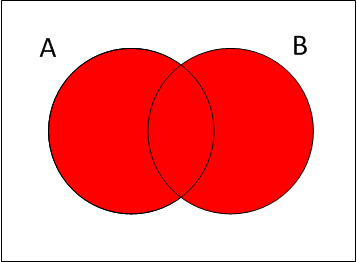
\includegraphics[width=1.5in]{test08-2a.png}
\end{center}
\end{minipage}
\end{tabular}


\begin{tabular}{@{}ll@{}} 
\begin{minipage}{0.7\columnwidth}
\begin{uzdevums}[nt.divisor-structure.03]
% AOPS.INT.5.3a
(Ieslēgšanas-izslēgšanas princips). Cik ir skaitļu no $1$ līdz $60$, kuri dalās 
ar vismaz vienu no skaitļiem $2$, $3$ vai $5$? 
Pēterītis izrēķināja, ka ${\displaystyle 60 \cdot \left( 1 - \frac{1}{2} \right)
 \cdot \left( 1 - \frac{1}{3} \right) \cdot \left( 1 - \frac{1}{5} \right) = 16}$. 
Viņš apgalvo, ka tas sakrīt ar to skaitļu skaitu no 
$1$ līdz $60$, kuri nedalās ne ar $2$, ne ar $3$, ne ar $5$. Vai Pēterītim taisnība?
\end{uzdevums}
\end{minipage} &
\begin{minipage}{0.25\columnwidth}
\begin{center}
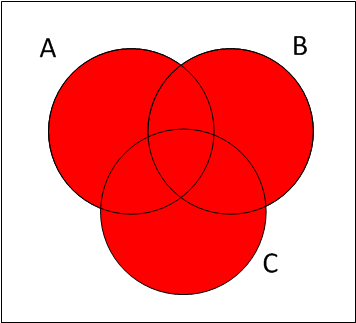
\includegraphics[width=1.5in]{test08-3a.png}
\end{center}
\end{minipage}
\end{tabular}





%% PAŅEMTS uz DUDAJEVAGATVE.LV
\begin{uzdevums}[nt.divisor-structure.04]
% AOPS.INT.5.2
Planētām $X$, $Y$ un $Z$ vajag attiecīgi $360$, $450$ un $540$ dienas, lai veiktu pilnu apli ap to pašu 
sauli. Ja visas trīs planētas sākumā ir sarindojušās uz tā paša stara (kuram saule ir sākumpunkts), 
kāds ir mazākais pozitīvais dienu skaits, pirms viņas nonāks šajā pašā sākuma stāvoklī? 
\end{uzdevums}


\begin{uzdevums}[nt.divisor-structure.05]
% AOPS.INT.5.3
Ar $\gcd(a, b)$ apzīmēsim skaitļu $a$ un $B$ lielāko kopīgo dalītāju, un 
ar $\operatorname{lcm}(c,d)$ apzīmēsim mazāko kopīgo dalāmo skaitļiem $c$ un $d$. 
Cik ir $\gcd(\operatorname{lcm}(8,14),\operatorname{lcm}(7,12))$?
\end{uzdevums}

%% PAŅEMTS uz DUDAJEVAGATVE.LV
\begin{uzdevums}[nt.divisor-structure.06]
% AOPS.INT.5.4
Ar $A$ apzīmējam visus tos skaitļus, ko var izteikt kā triju pēc kārtas sekojošu naturālu skaitļu summu. 
Kāds ir lielākais kopīgais dalītājs visiem skaitļiem kopā $A$? 
\end{uzdevums}


\begin{uzdevums}[nt.divisor-structure.07]
% AOPS.INT.5.5
Kāds ir lielākais kopīgais dalītājs skaitļiem $7979$ un $3713$? (Ieteicams no lielākā skaitļa atņemt kādu mazākā skaitļa 
daudzkārtni, pēc tam - lielāko skaitli aizstāt ar atlikumu, utt.). 
\end{uzdevums}

\begin{uzdevums}[nt.divisor-structure.08]
% AOPS.INT.5.2.3
Karlīne novieto 600 lodītes $m$ kastēs tā, lai katrā kastē būtu vienāds skaits lodīšu. 
Ir vairāk nekā viena kaste, un katrā kastē ir vairāk nekā viena lodīte. 
Cik dažādām $m$ vērtībām Karlīne to var izdarīt? 
\end{uzdevums}

%% PAŅEMTS uz DUDAJEVAGATVE.LV
\begin{uzdevums}[nt.divisor-structure.09]
% AOPS.INT.5.4
Cik daudzi no skaitļa 168 pozitīvajiem dalītājiem ir pāru skaitļi?
\end{uzdevums}

%% PAŅEMTS uz DUDAJEVAGATVE.LV
\begin{uzdevums}[nt.divisor-structure.10]
% AOPS.INT.5.6
Cik daudzi no skaitļa $5400$ dalītājiem nav daudzkārtņi nevienam pilnam kvadrātam lielākam par $1$? 
\end{uzdevums}





\end{document}